\section{Optimizing Object Tracking}
\label{sec:methods/section_b}

Object tracking pipeline consists of YOLOv3 and SORT, and using the software from \cite{jocher_ultralyticsyolov3_2021} and \cite{abewley_abewleysort_2021}, there are 6 parameters to be set to run object tracking. We set the appropriate parameters by optimizing the detection performance of YOLOv3 and tracking performance of SORT. The following are the parameters that need to be set for YOLOv3.
\begin{itemize}
    \item \textbf{Image size}: This is the image resolution to which input image will be resized prior to being input to the YOLOv3 model.
    \item \textbf{Confidence threshold}: This is the minimum confidence needed to declare a detected object. The higher the threshold, the object detector will be less likely to detect the target but fewer mistakes will be made in detection.
    \item \textbf{IOU threshold for Non-maximum suppression (NMS)}: NMS prevents multiple detections on the same target \cite{redmon_you_2016}. IOU threshold is used in applying NMS in our YOLOv3.
\end{itemize}
For image size, any input image will be resized to this resolution for prediction. Since the resolution of $640\times640$ was the largest resolution for which the pre-trained network weights are available, we speculated that the detection performance would be best with this particular resolution. Therefore, we chose $640\times 640$ as the image size, which is also a default value provided by the software \cite{jocher_ultralyticsyolov3_2021}.

For the confidence threshold and IOU threshold for NMS, we apply the grid search to determine the suitable values. To tune these parameters, we run YOLOv3 and SORT on the sequence PartyScene. Subsequently, this sequence will not be used in testing tracking accuracy. Since both parameters range from 0 to 1, we run the detector with a step size of 0.05 and plot the detection F1 score over different confidence thresholds and IOU thresholds as shown in Figure \ref{fig:optimizing_detector}.
%https://tex.stackexchange.com/questions/278574/common-caption-below-vertically-centered-figure-and-table

\begin{figure}[!tb]
\centering

\begin{tabular}{@{}c@{}}
\resizebox{0.5\linewidth}{!}{
  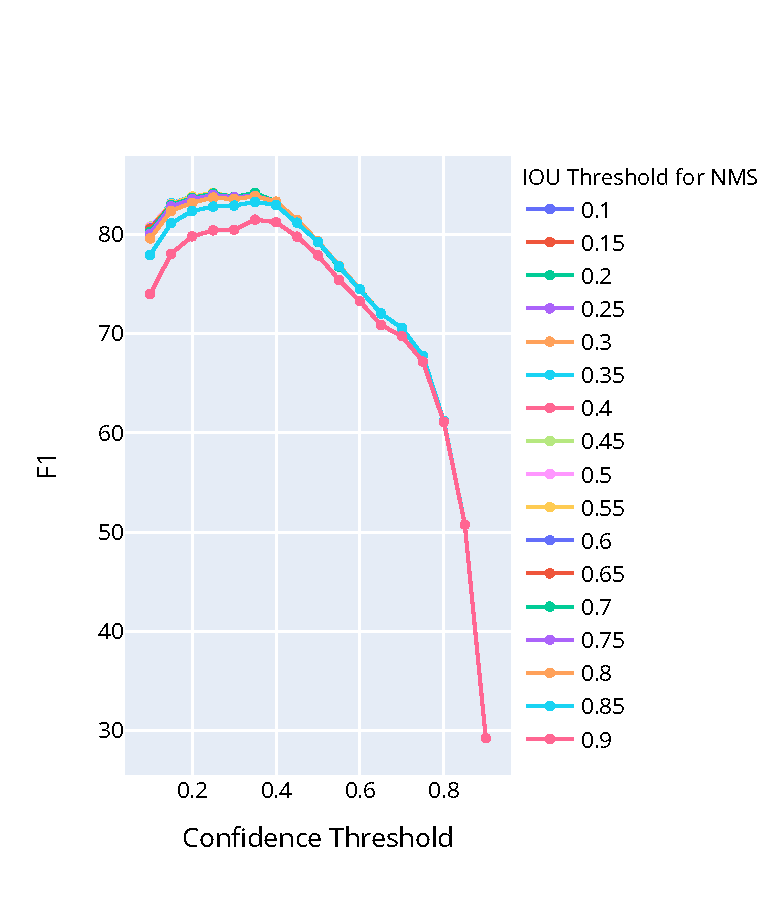
\includegraphics{img/optimizing_detector.pdf}}
\end{tabular}\qquad
\resizebox{0.4\linewidth}{!}{
\begin{tabular}{rrr}
\toprule
 Confidence Threshold &  IOU threshold for NMS &    F1 \\
\midrule
                 0.25 &                   0.35 & 84.20 \\
                 0.25 &                   0.40 & 84.20 \\
                 0.25 &                   0.45 & 84.20 \\
                 0.25 &                   0.50 & 84.20 \\
                 0.25 &                   0.55 & 84.20 \\
\bottomrule
\end{tabular}
}

\caption[Optimizing YOLOv3 by maximizing F1 score on "all" object classes]
{Optimizing YOLOv3 by maximizing F1 score on "all" object classes.}
\label{fig:optimizing_detector}
\end{figure}
The table and plot in this figure show that there are optimal F1 scores over different confidence and IOU threshold values. The table with the plot shows that the detector achieved the same F1 score over different IOU thresholds at a confidence threshold of 0.25. The default threshold values provided by the software \cite{jocher_ultralyticsyolov3_2021} are a confidence threshold of 0.25 and IOU threshold of 0.45. Since the higher the IOU threshold we choose, it makes the detector more careful in detection (in other words, we expect to see less FP and more FN), so we chose the confidence threshold of 0.25 and the IOU threshold for NMS to be 0.55.

For optimizing the tracking performance of SORT, the following input parameters were considered \cite{bewley_simple_2016}.
\begin{itemize}
    \item \textbf{Max age}: Denoted T\textsubscript{lost} as explained in section \ref{sec:background/section_b}, the value of maximum age determines the maximum number of frames for a trajectory to be alive while no objects are detected before its termination.
    \item \textbf{Min hits}: Minimum number of necessary detections before the trajectory creation and its assignment initialization.
    \item \textbf{IOU threshold}: Minimum IOU threshold for object matching. IOU less than this threshold indicates that the object does not overlap enough with the ground truth, so identity will not be assigned, but an assignment occurs when IOU is higher than the threshold.
\end{itemize}
For the max age, we chose the value of 1 because \citeauthor{bewley_simple_2016} \cite{bewley_simple_2016} justified this value by the two reasons; the constant linear motion in the Kalman filter framework does not cover the true dynamics where the non-linear motion exists, and SORT does not deal with object re-identification. The max age of 1 is also a default value provided by their software \cite{abewley_abewleysort_2021}. 

For the min hits and IOU threshold, we run SORT on the training sequence PartyScene for both parameters from 0.1 to 0.9 at a step size of 0.05 as a grid search. To optimize these parameters, we have tested both single-class of "person" tracking, and "all" object classes as multi-class tracking. We have chosen "person" for single-class tracking in this tuning since it is an important special case. For the "all" object classes tracking case, SORT will track all object classes available in the ground truth. Figure \ref{fig:optimizing_tracker_0} shows the result of "person" class tracking. The evaluation based on MOTA over different min hits and IOU thresholds is plotted, and the highest scores are shown in the table. Although there is no single metric that has been agreed to evaluate the tracking performance, MOTA is the most popular metric in MOT and serves as a good indicator for the general tracking performance \cite{milan_mot16_2016} \cite{bernardin_evaluating_2008}. Therefore, we optimized based on MOTA instead of solving multiple objective optimization problem for all the performance metrics. This result indicates that for "person" tracking, the MOTA score is optimal at min hits of 2 and the IOU threshold from 0.10 to 0.40. Figure \ref{fig:optimizing_tracker_all} which corresponds to tracking "all" object classes shows that min hits of 9 and IOU threshold from 0.10 to 0.40 achieve the optimal performance.
\begin{figure}[htbp]
  \centering
 
  \begin{subfigure}{1.0\textwidth}
\centering

    \begin{tabular}{@{}c@{}}
    \resizebox{0.5\linewidth}{!}{
      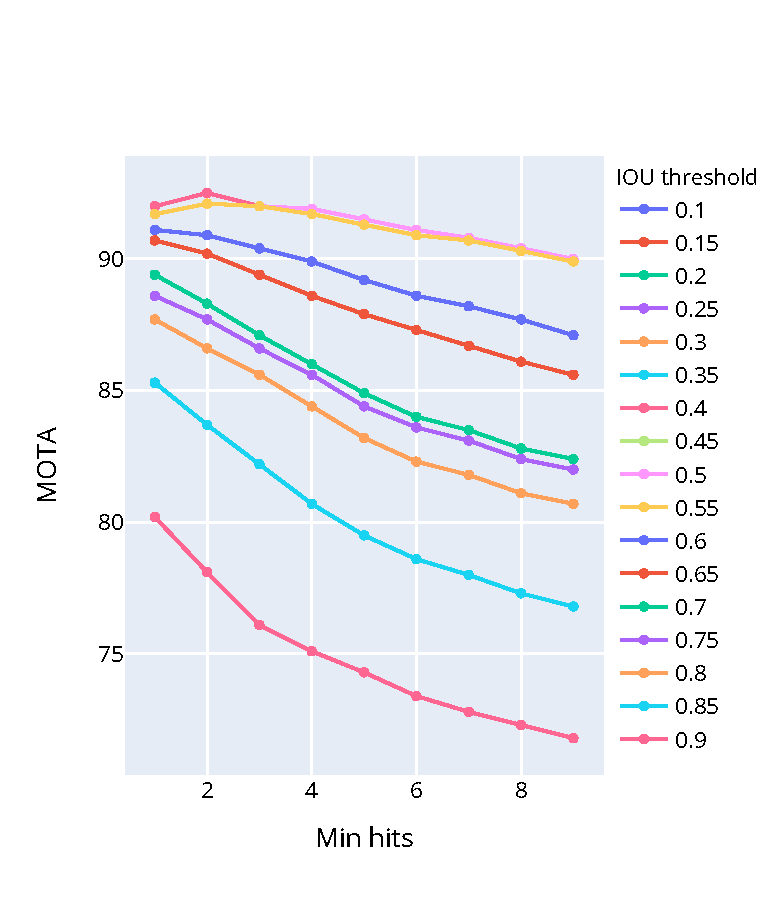
\includegraphics{img/optimizing_tracker_0.pdf}}
    \end{tabular}\qquad
    \resizebox{0.4\linewidth}{!}{
    \begin{tabular}{rrrr}
    \toprule
     Max age &  Min hits & IOU threshold &  MOTA \\
    \midrule
           1 &         2 &       0.10 & 92.50 \\
           1 &         2 &       0.15 & 92.50 \\
           1 &         2 &       0.20 & 92.50 \\
           1 &         2 &       0.25 & 92.50 \\
           1 &         2 &       0.30 & 92.50 \\
           1 &         2 &       0.35 & 92.50 \\
           1 &         2 &       0.40 & 92.50 \\
    \bottomrule
    \end{tabular}
    }
    
    \caption{A caption for a figure in a figure and a table side by side}\label{fig:optimizing_tracker_0}
  \end{subfigure}
 
    \bigskip
 
  \begin{subfigure}{1.0\linewidth}
    \centering
    
    \begin{tabular}{@{}c@{}}
    \resizebox{0.5\linewidth}{!}{
      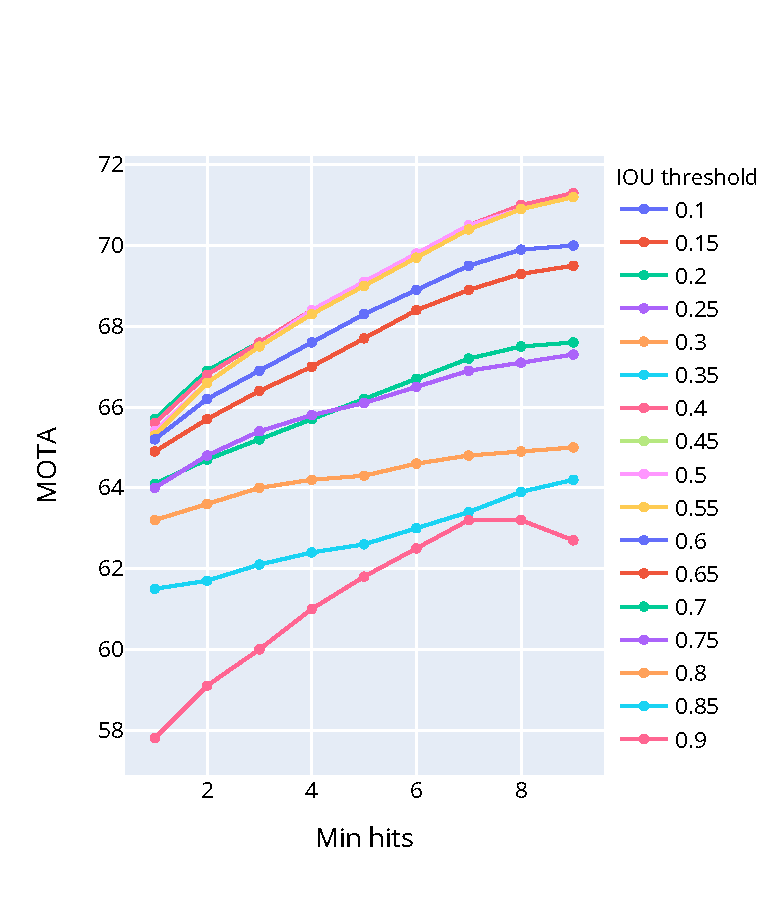
\includegraphics{img/optimizing_tracker_all.pdf}}
    \end{tabular}\qquad
    \resizebox{0.4\linewidth}{!}{
    \begin{tabular}{rrrr}
    \toprule
     Max age &  Min hits &  IOU threshold &  MOTA \\
    \midrule
           1 &         9 &       0.10 & 71.30 \\
           1 &         9 &       0.15 & 71.30 \\
           1 &         9 &       0.20 & 71.30 \\
           1 &         9 &       0.25 & 71.30 \\
           1 &         9 &       0.30 & 71.30 \\
           1 &         9 &       0.35 & 71.30 \\
           1 &         9 &       0.40 & 71.30 \\
    \bottomrule
    \end{tabular}
    }
    
    \caption{A caption for a figure in a figure and a table side by side}\label{fig:optimizing_tracker_all}
  \end{subfigure}
  

  \caption{}
  \label{fig:optimizing_tracker} % label should be placed below caption
\end{figure}
Note that the default values are min hits of 3 and IOU threshold of 0.3 provided by the software \cite{abewley_abewleysort_2021}, and \citeauthor{bewley_simple_2016} \cite{bewley_simple_2016} used these values to only track the "person" object class. Using these default values in our sequence PartyScene, we got MOTA score of 92.00 on the "person" object class and 67.60 on the "all" object classes, which are slightly lower than our optimal MOTA scores of 92.50 and 71.30 for both tracking cases respectively. Based on these results, we chose 0.4 for the IOU threshold since both tracking cases, single-class of "person" tracking and multi-class tracking, give the best MOTA score at the IOU threshold up to 0.4, and the higher the IOU threshold, the more careful design the tracker is. For the min hits, we chose the value of 5, which is roughly halfway between 2 and 9, taking both single-class and multi-class tracking into consideration.

As we have selected the values of three parameters based on MOTA (max age of 1, min hits of 5, and IOU threshold of 0.4), the further justification for other metrics is given in the Appendix \ref{sec:appendix/section_a}. The selected values of parameters in YOLOv3 and SORT are summarized in Table \ref{tab:parameters}.
\begin{table}[!htbp]
    \centering
    \resizebox{0.4\linewidth}{!}{
    \begin{tabular}{r|r}
    \hline
    YOLOv3 Parameter &  Selected value \\
    \hline
         Image size &               640x640 \\
         Confidence threshold &     0.25 \\
         IOU threshold for NMS &    0.55 \\
    \hline
         SORT Parameter &           Selected value \\
    \hline
         Max age &                  1 \\
         Min hits &                 5 \\
         IOU threshold for matching & 0.4 \\
    \hline
    \end{tabular}
    }
    \caption{Caption}
    \label{tab:parameters}
\end{table}